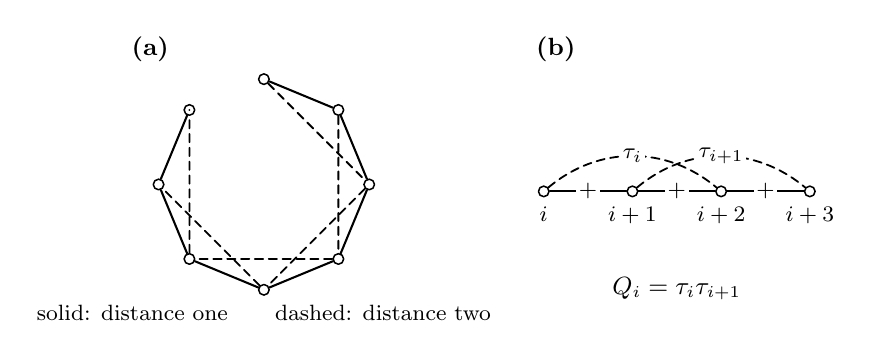
\begin{tikzpicture}[
  x=0.88cm,
  y=0.88cm,
  line cap=round,
  line join=round,
  vertex/.style={circle,draw=black,fill=white,inner sep=1.35pt,
    line width=0.55pt},
  stepone/.style={draw=black,line width=0.75pt},
  steptwo/.style={draw=black,densely dashed,line width=0.65pt},
  signlabel/.style={fill=white,inner sep=1pt,font=\footnotesize},
  panel/.style={font=\small\bfseries,anchor=west}
]
  % (a) The full graph C_8^2.
  \node[panel] at (-0.35,3.50) {(a)};
  \node[vertex] (a0) at (1.70,3.07) {};
  \node[vertex] (a1) at (2.775,2.625) {};
  \node[vertex] (a2) at (3.22,1.55) {};
  \node[vertex] (a3) at (2.775,0.475) {};
  \node[vertex] (a4) at (1.70,0.03) {};
  \node[vertex] (a5) at (0.625,0.475) {};
  \node[vertex] (a6) at (0.18,1.55) {};
  \node[vertex] (a7) at (0.625,2.625) {};
  \draw[stepone]
    (a0)--(a1)--(a2)--(a3)--(a4)--(a5)--(a6)--(a7)--cycle;
  \draw[steptwo]
    (a0)--(a2)--(a4)--(a6)--cycle
    (a1)--(a3)--(a5)--(a7)--cycle;
  \node[font=\footnotesize] at (1.70,-0.30)
    {solid: distance one\qquad dashed: distance two};

  % (b) Local Hamilton-gauge coordinates.
  \begin{scope}[xshift=5.05cm]
    \node[panel] at (-0.25,3.50) {(b)};
    \foreach \k/\lab in {0/i,1/{i+1},2/{i+2},3/{i+3}} {
      \node[vertex,label={[font=\footnotesize]below:$\lab$}]
        (b\k) at ({1.28*\k},1.45) {};
    }
    \draw[stepone] (b0)--(b1)--(b2)--(b3);
    \node[signlabel] at (0.64,1.45) {$+$};
    \node[signlabel] at (1.92,1.45) {$+$};
    \node[signlabel] at (3.20,1.45) {$+$};
    \draw[steptwo,bend left=40] (b0) to
      node[signlabel,pos=0.5] {$\tau_i$} (b2);
    \draw[steptwo,bend left=40] (b1) to
      node[signlabel,pos=0.5] {$\tau_{i+1}$} (b3);
    \node[font=\small] at (1.92,0.05)
      {$Q_i=\tau_i\tau_{i+1}$};
  \end{scope}
\end{tikzpicture}
